% ============================================================
% LLM-BLM プロジェクト総合報告書 2（総合報告書 1〔2026-10-13 版〕の後の作業）
% コンパイル：tectonic -X compile LLM-BLM_総合報告書2.tex   （XeTeX 系。このフォルダで実行する）
% 図は LLM-BLM_総合報告書2_図/（作成スクリプト/collect.py が各実験の図を集める）
% 文字は原ノ味（総合報告書 1 のヒラギノは Windows にないため）
% ============================================================
\documentclass[xelatex,ja=standard,jafont=haranoaji,a4paper,10pt]{bxjsreport}
\setpagelayout*{left=25mm,right=25mm,top=28mm,bottom=28mm,footskip=12mm}

\usepackage{amsmath,amssymb}
\usepackage{booktabs,longtable,array,multirow}
\usepackage{graphicx}
\usepackage{adjustbox}
\usepackage{xcolor}
\usepackage{tikz}
\usetikzlibrary{arrows.meta,positioning,calc,fit}
\usepackage{enumitem}
\usepackage{caption}
\usepackage{float}
\usepackage[most]{tcolorbox}
\usepackage[hidelinks,bookmarksnumbered]{hyperref}
\pdfstringdefDisableCommands{\def\Omega{Ω}\def\Sigma{Σ}}

\graphicspath{{LLM-BLM_総合報告書2_図/}}

% ---- 色
\definecolor{c1}{HTML}{2A78D6}
\definecolor{c2}{HTML}{EB6834}
\definecolor{c3}{HTML}{1BAF7A}
\definecolor{c4}{HTML}{EDA100}
\definecolor{c7}{HTML}{6250D6}
\definecolor{ink2}{HTML}{52514E}
\definecolor{soft1}{HTML}{E4EEF9}
\definecolor{soft2}{HTML}{FBEEDF}
\definecolor{soft3}{HTML}{E3F3E9}
\definecolor{soft4}{HTML}{EEE8FA}
\definecolor{soft5}{HTML}{FBE6E6}

% ---- よく使う表記
\newcommand{\SP}{S\&P500}
\newcommand{\code}[1]{\texttt{#1}}
\newcommand{\figref}[1]{図~\ref{#1}}
\newcommand{\tabref}[1]{表~\ref{#1}}
\newcommand{\chapref}[1]{第~\ref{#1}~章}
\newcommand{\secref}[1]{\ref{#1}~節}

% ---- リスト
\setlist[itemize]{leftmargin=1.6em,itemsep=0.2em,topsep=0.4em}
\setlist[enumerate]{leftmargin=1.8em,itemsep=0.2em,topsep=0.4em}

% ---- 表と図
\captionsetup{font=small,labelfont=bf,skip=6pt}
\renewcommand{\arraystretch}{1.25}
\setlength{\LTpre}{6pt}
\setlength{\LTpost}{6pt}

% ---- 要点の囲み
\newtcolorbox{keybox}[1][要点]{enhanced,breakable,colback=soft1,colframe=c1,boxrule=0.5pt,arc=2pt,
  left=8pt,right=8pt,top=6pt,bottom=6pt,title={#1},fonttitle=\sffamily\bfseries\small,coltitle=white}
\newtcolorbox{notebox}[1][注意]{enhanced,breakable,colback=soft2,colframe=c2,boxrule=0.5pt,arc=2pt,
  left=8pt,right=8pt,top=6pt,bottom=6pt,title={#1},fonttitle=\sffamily\bfseries\small,coltitle=white}
\newtcolorbox{verdict}[1][判定]{enhanced,breakable,colback=soft4,colframe=c7,boxrule=0.5pt,arc=2pt,
  left=8pt,right=8pt,top=6pt,bottom=6pt,title={#1},fonttitle=\sffamily\bfseries\small,coltitle=white}

% ---- 図の部品
\tikzset{
  box/.style={draw=#1,fill=#1!12,rounded corners=2pt,align=center,inner sep=5pt,font=\small,minimum height=9mm},
  box/.default=c1,
  arr/.style={-{Stealth[length=2mm]},line width=0.6pt,color=ink2},
  lab/.style={font=\scriptsize,color=ink2}
}

\begin{document}

% ============================================================
% 表紙
% ============================================================
\hypersetup{pdftitle={LLM-BLM プロジェクト総合報告書 2},pdfauthor={小嶋 一輝},pageanchor=false}
\begin{titlepage}
\centering
\vspace*{30mm}
{\sffamily\Large 情報工学工房　プロジェクト総合報告書 2\par}
\vspace{14mm}
{\sffamily\bfseries\huge LLM の数値予想から、\par\vspace{3mm}決算発表文の読み取りへ\par}
\vspace{12mm}
{\large 仮説の検証、方針の見直し、文献調査、\par\vspace{2mm}新しいアーキテクチャと事前登録した実験の記録\par}
\vspace{30mm}
{\large 電気通信大学　情報理工学域 III 類\par}
\vspace{3mm}
{\Large 小嶋 一輝\par}
\vspace{20mm}
{\large 2026 年 10 月 18 日 版\par}
\vfill
{\small 総合報告書 1（2026 年 10 月 13 日 版）の続き。対象の期間は 2026 年 10 月 14 日から 18 日。\par}
\end{titlepage}
\hypersetup{pageanchor=true}

% ============================================================
% 概要
% ============================================================
\chapter*{概要}
\addcontentsline{toc}{chapter}{概要}

本書は、総合報告書 1（2026 年 10 月 13 日 版）の後、10 月 14 日から 18 日までに行った作業をまとめたものである。総合報告書 1 は、元論文（Lee ほか、arXiv:2504.14345）の計算を再現し、問題点を確かめ、「gpt-4o-mini の答えは、渡した数字の中の直近の値動きに沿う」ことを 7 つの実験で示した。本書の作業は 4 つに分かれる。

\begin{enumerate}
\item \textbf{仮説の検証（H01〜H07）}：総合報告書 1 の課題を 7 つの仮説に分け、事前に決めた指標と判定の基準で検証した。結果は、別の 2 つのモデル（Codex と Gemini）にも読ませて確かめた。
\item \textbf{方針の見直しと文献調査}：次に何をするかの方針を、Claude・GPT・Gemini の 3 者に独立に書かせて比べた。先行研究は、Gemini Deep Research を加えた 4 者で調べ、挙がった文献をすべて機械的に照合した。
\item \textbf{新しいアーキテクチャ}：LLM の役割を「決算発表文から判断を読み取ること」に絞り、決算発表 1 本を単位にする評価の仕組み（DB の表、時刻の規則、5 つの点数の付け方）を設計して実装した。2015〜2026 年の決算発表 28,447 本を取得し、先読みのない ChronoGPT の環境も作った。
\item \textbf{事前登録した実験（実験 2）}：評価の手順と判定の基準を、株価の反応を計算する前に文書とコードで固定し、1 回だけ実行した。
\end{enumerate}

\begin{keybox}[本書の主な結論]
\begin{itemize}
\item \textbf{LLM に数値のリターンを予想させる構成には、価値がない。}予想の 81\% は渡した月の値動きの写しで、写しを除いた固有の IC は $-0.004$ だった。BLM の計算は、当たり具合で $\Omega$ を較正すれば設計どおりに動くが、成績は予想を並べ替えたビューと区別できなかった（H02、H04）。
\item \textbf{LLM が決算発表文から読み取った点数は、発表への株価の反応をはっきり説明する（実験 2、事前登録した検定で支持）。}点数が 1 標準偏差高いと、発表をはさむ 2 取引日の超過リターンは $+1.20\%$ 高い（$t$ 9.4、置換の対照で $p=0.001$）。辞書・FinBERT・TF-IDF・数値の驚きを統制しても変わらず、効果は FinBERT や TF-IDF の約 3 倍だった。
\item \textbf{ただし、取引にも BLM のビューにも使えない。}反応は発表の 2 日のうちに出尽くし、その後のドリフトは有意でない。点数が手に入るときには、株価はすでに動いている。
\item \textbf{先読みのない小さなモデル（ChronoGPT）は、質問に答えさせる使い方ではほとんど読み取れない}（同じ標本で $+0.04\%$）。
\item 方法の面では、(1) 3 者の方針の比較、(2) 文献の機械的な照合（どのモデルの文献にも誤りがあった）、(3) 事前登録、の 3 つが、結論の確かさを支えた。
\end{itemize}
\end{keybox}

本書の数値は、とくに断りがなければ、リポジトリのブランチ \code{feature/earnings-events}（実験 2）と \code{research/llm-blm-results-report}（H01〜H07）の結果のファイルから取った。詳しい報告は『LLM-BLM 実験結果レポート』（H01〜H07）と『LLM-BLM 実験 2』にある。

\setcounter{tocdepth}{1}
\tableofcontents

% ============================================================
\part{背景}
% ============================================================

\chapter{総合報告書 1 の後に残っていた問い}\label{ch:intro}

総合報告書 1 の結論は、次の 3 つだった。

\begin{itemize}
\item 元論文の計算では、BLM が LLM の予想を中央値で 99.9\% 採用し、市場の均衡がほとんど使われていない。最適化（SLSQP）も途中で止まっている。
\item gpt-4o-mini の予想は、渡した月の平均リターンとの相関が 0.89 で、翌月の実際のリターンとの順位相関は $+0.05$ にとどまる。
\item 入力や質問の形を変えた 7 つの実験でも、LLM は渡した数字の中の直近の値動きをなぞった。数字の処理は統計モデルに任せ、LLM には文章の解釈だけをさせる構成を、次に確かめるべきである。
\end{itemize}

残っていた問いは、(a) LLM の予想に「なぞり」以外の情報が少しでもあるか、(b) BLM の設計（$q$、$P$、$\Omega$）をどう直せばよいか、(c) 文章を読ませれば違うか、(d) フィードバックで良くなるか、の 4 つである。

\section{作業の流れ}

\begin{figure}[H]
\centering
\begin{tikzpicture}[node distance=5mm and 6mm]
\node[box=c1,text width=26mm] (a) {仮説の検証\\H01〜H07\\{\scriptsize 10/14〜16}};
\node[box=c4,text width=26mm,right=of a] (b) {方針の見直し\\3 者の比較\\{\scriptsize 10/17}};
\node[box=c4,text width=26mm,right=of b] (c) {文献調査\\4 者＋照合\\{\scriptsize 10/17}};
\node[box=c3,text width=26mm,below=of c] (d) {新しい\\アーキテクチャ\\{\scriptsize 10/17}};
\node[box=c3,text width=26mm,left=of d] (e) {データと点数\\28,447 本\\{\scriptsize 10/17〜18}};
\node[box=c7,text width=26mm,left=of e] (f) {事前登録と\\実験 2\\{\scriptsize 10/18}};
\draw[arr] (a) -- (b); \draw[arr] (b) -- (c); \draw[arr] (c) -- (d); \draw[arr] (d) -- (e); \draw[arr] (e) -- (f);
\end{tikzpicture}
\caption{本書の作業の流れ。}
\end{figure}

\section{本書の読み方}

\begin{itemize}
\item 第 II 部は、『実験結果レポート』の要約である。数値と判定はそのレポートと同じで、詳細はそちらにある。
\item 第 III 部は、方針と文献調査の記録である。元の文書は \code{資料集/03\_方針と文献調査/} にある。
\item 第 IV・V 部は、新しいアーキテクチャと実験 2 である。『実験 2』のレポートより、設計と実装の説明を詳しくした。
\end{itemize}

% ============================================================
\part{仮説の検証（H01〜H07）}
% ============================================================

\chapter{仮説と方法}\label{ch:hyp}

総合報告書 1 の課題を、7 つの仮説に分けた（『LLM-BLM 実験仮説』）。仮説ごとに Git のブランチを分け、指標・判定の基準・使うデータを、実行の前に決めた。

\begin{table}[H]
\centering
\caption{7 つの仮説。}
\small
\begin{tabular}{lp{9.5cm}r}
\toprule
ID & 内容 & API \\
\midrule
H01 & 現行の計算の再現と整合性 & なし \\
H02 & LLM の数値予想は、入力の写しと統計モデルを超える情報を持つか & なし \\
H03 & ビューの形（絶対・相対・順位）で、ベータへの傾きが消えるか & なし \\
H04 & $\Omega$：回答の分散、過去の当たり具合による較正、縮小、置換による対照 & なし \\
H05 & 市場とセクターを、文章だけ・数字だけで聞く & 1,080 回 \\
H06 & 決算発表文から LLM が判断を取り出し、統計で数値化する & 5,429 回 \\
H07 & 過去の成績をフィードバックする LLM & 約 11,600 回 \\
\bottomrule
\end{tabular}
\end{table}

共通の条件は次のとおりである。

\begin{itemize}
\item 評価期間は 2024 年 3 月末〜2026 年 8 月末の判断日 30 か月。gpt-4o-mini の知識の期限（2023 年 10 月）より後。
\item 対象は各時点の \SP{} の構成銘柄（月平均 489 銘柄）。
\item 比率の計算は、TE の上限つきの平均分散最適化（Clarabel）。売買のコストは片道 0.1\%。
\item API の費用は合計 6.72 ドル（18,237 リクエスト）。
\end{itemize}

\chapter{結果}\label{ch:hresult}

\section{H01：計算の再現}

資料の数値はほぼすべて再現できた。ただし、元論文の最適化（SciPy の SLSQP）は、入力のごく小さな違いで止まる位置が変わり、比率を再現できなかった（\figref{fig:h01}）。

\begin{figure}[H]
\centering
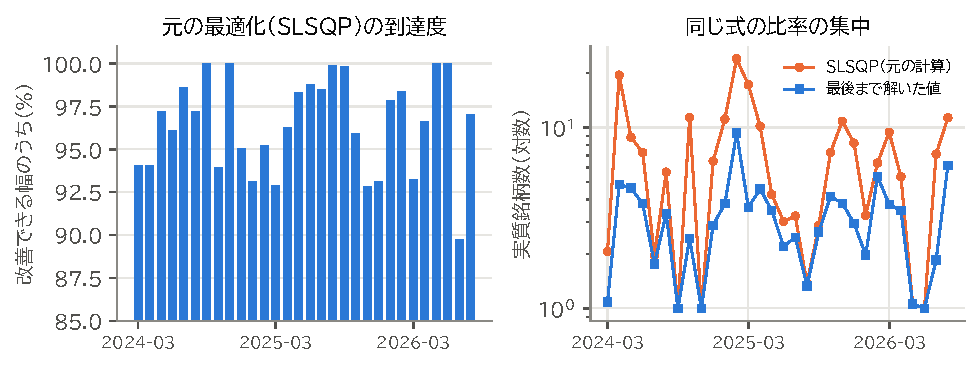
\includegraphics[width=0.88\linewidth]{h01_slsqp.pdf}
\caption{左：元の最適化が、改善できる幅の何 \% まで進んで止まったか。右：同じ目的関数の比率の集中（SLSQP の結果と、最後まで解いた結果）。}
\label{fig:h01}
\end{figure}

\section{H02：LLM の数値予想は、入力の写し}

LLM の予想の 81\% は、渡した月の平均と散らばりの直線の関数で説明できた。写しを除いた LLM に固有の部分の IC は $-0.004$（95\% 区間 $-0.036$〜$+0.027$）。LLM と同じ当たり具合（IC $+0.05$）は、「先月の平均リターン」をそのまま使っても得られる（\figref{fig:h02}）。\textbf{支持された}（固有の予測力は、あっても IC 0.03 未満）。

\begin{figure}[H]
\centering
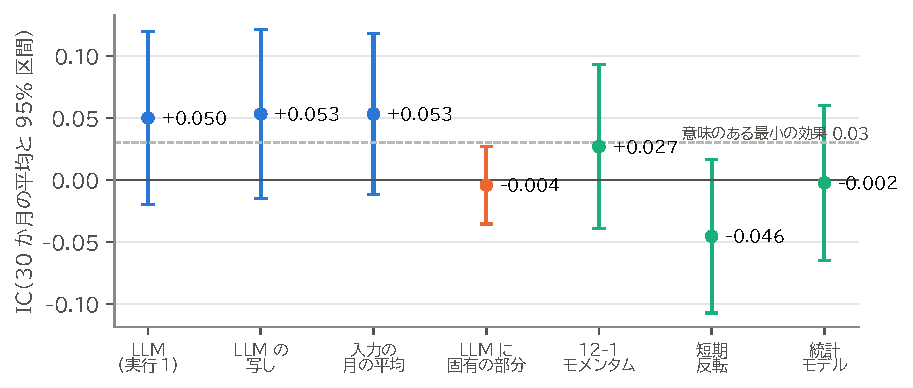
\includegraphics[width=0.88\linewidth]{h02_ic.pdf}
\caption{予想ごとの IC（30 か月の平均と 95\% 区間）。}
\label{fig:h02}
\end{figure}

\section{H03：相対ビューでも、ベータへの傾きは消えない}

市場が上がった月には高ベータの銘柄が上がり、LLM がそれをなぞるので、銘柄の間の予想の差そのものがベータに傾く。相対ビューにしても、能動ベータは 0.94 倍にしか減らなかった（\figref{fig:h03}）。\textbf{支持されなかった}。

\begin{figure}[H]
\centering
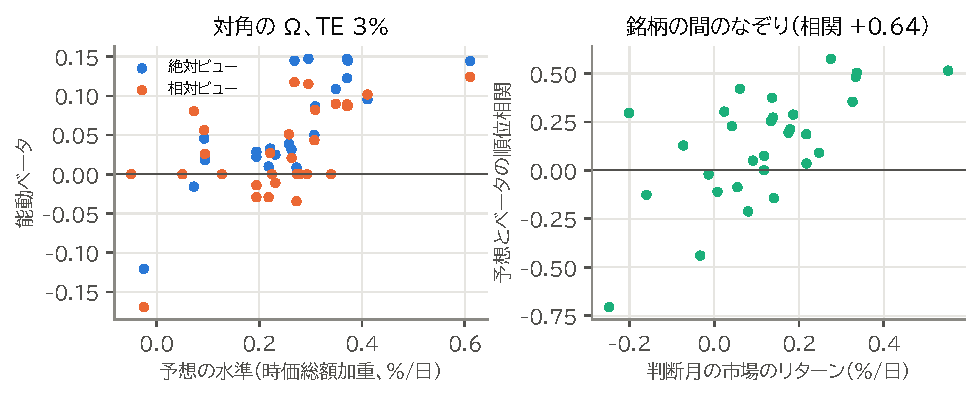
\includegraphics[width=0.88\linewidth]{h03_beta.pdf}
\caption{左：予想の水準と能動ベータ（30 か月）。右：判断日ごとの「LLM の予想と銘柄のベータの順位相関」と、判断月の市場のリターン。}
\label{fig:h03}
\end{figure}

\section{H04：較正した BLM は設計どおりに動くが、成績は偶然と区別できない}

$\Omega\propto\Sigma$ とし、採用率を判断日より前の較正の傾き（推定の誤差で縮めたもの）にすると、BLM は設計どおりに動いた。採用率は設定どおり、比率は時価総額加重を少し動かす形（実質 47 銘柄、実績の TE 4.2\%）になった。しかし成績（コスト控除後 年率 $+0.53\%$）は、予想を銘柄の間で並べ替えたビュー 200 回と区別できない（片側 $p=0.104$。セクターの中だけで並べ替える厳しい対照では 0.38）（\figref{fig:h04}）。回答のばらつきは、誤差の大きさとしては確信が強すぎて使えない（外れの 2 乗の約 8 分の 1）が、外れやすさの順番の手がかりにはなった（偏順位相関 $+0.17$）。

\begin{figure}[H]
\centering
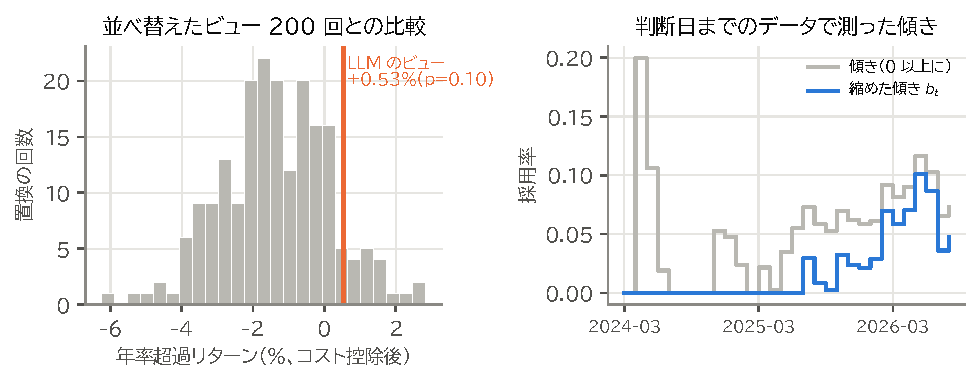
\includegraphics[width=0.88\linewidth]{h04_placebo.pdf}
\caption{左：並べ替えたビュー 200 回の超過リターンの分布と、実際の LLM のビュー。右：判断日までのデータで測った較正の傾き（灰）と、推定の誤差で縮めた値（青）。}
\label{fig:h04}
\end{figure}

\section{H05：文章だけを渡すと、なぞりが消える}

月次レポートの文章だけを渡すと、市場の点数と直近 1 か月のリターンの順位相関が $+0.77$ から $+0.05$ に下がった（\figref{fig:h05}）。ただし、セクターの判断が当たるかは、30 か月では確かめられなかった（IC $+0.06$、$t$ 0.72）。

\begin{figure}[H]
\centering
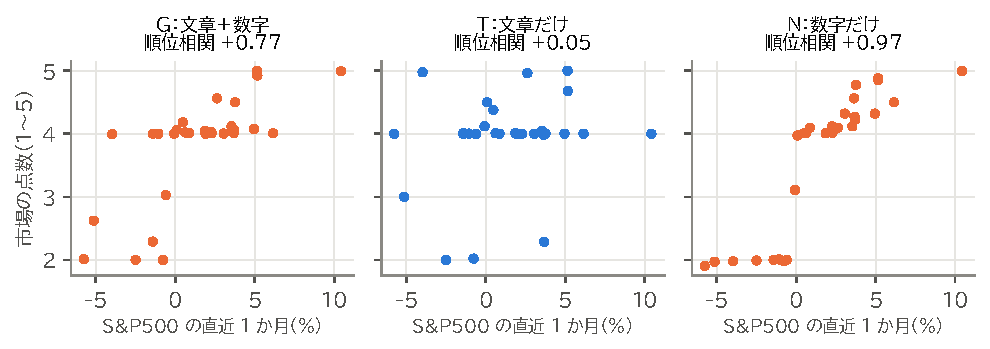
\includegraphics[width=0.95\linewidth]{h05_trace.pdf}
\caption{市場の点数と、\SP{} の直近 1 か月のリターン（30 か月）。左から、数字と文章（G）、文章だけ（T）、数字だけ（N）。}
\label{fig:h05}
\end{figure}

\section{H06：決算発表文の点数は、月次の検定では有意にならない}

決算発表文 5,429 本を gpt-4o-mini に読ませた点数は、直近の値動きをなぞらず（相関 $+0.08$）、業績の伸びに沿った（売上の前年比と $+0.41$）。しかし、翌月のリターンに対する事前に決めた検定（数値を統制した Fama--MacBeth の係数）は $t$ 0.97 で、\textbf{支持されなかった}。月ごとの IC の自己相関を考慮した Newey--West の $t$ では、IC $+0.033$ が $t$ 2.32 になり、探索的には有意だった（\figref{fig:h06}）。

\begin{figure}[H]
\centering
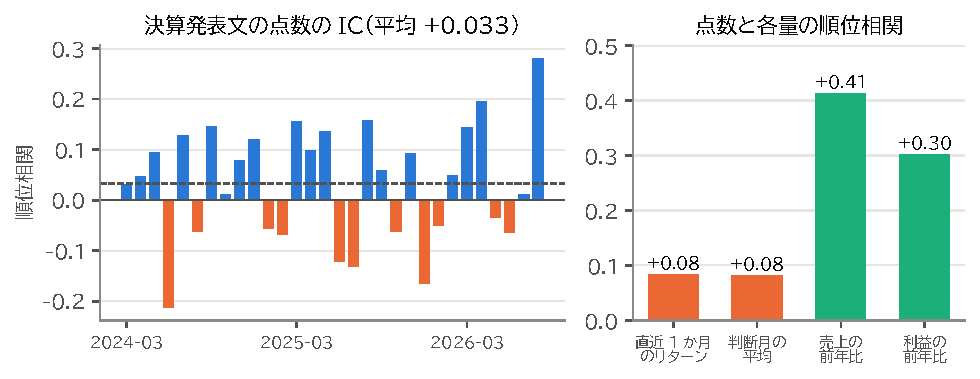
\includegraphics[width=0.88\linewidth]{h06_ic.pdf}
\caption{左：合成点数の月ごとの IC。右：合成点数と各量の順位相関（30 か月の平均）。}
\label{fig:h06}
\end{figure}

\section{H07：フィードバックで予想は良くならず、強気に寄る}

自分の過去の成績の要約を渡しても IC は上がらず（差 $+0.011$、$t$ 0.76）、楽観の偏りはかえって日次 $+0.12\%$ から $+0.29\%$ に強まった。どの月も一律に約 $+0.17\%$/日 上振れしており、要約を見せること自体が強気の目安として働いたと考えられる（\figref{fig:h07}）。\textbf{証拠不足}。

\begin{figure}[H]
\centering
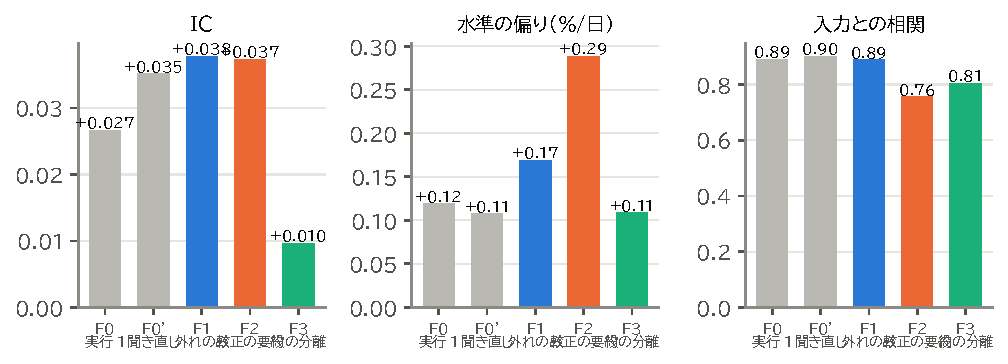
\includegraphics[width=0.95\linewidth]{h07_feedback.pdf}
\caption{条件ごとの IC、水準の偏り、入力との相関。}
\label{fig:h07}
\end{figure}

\section{判定のまとめ}

\begin{table}[H]
\centering
\caption{仮説ごとの判定（『実験結果レポート』の表と同じ）。}
\small
\begin{tabular}{llp{8.0cm}}
\toprule
ID & 判定 & 主な結果 \\
\midrule
H01 & 整合 & 式は一致。元の SLSQP は再現できない \\
H02 & 支持 & LLM に固有の IC $-0.004$ \\
H03 & 支持されず & 相対ビューでも能動ベータは 0.94 倍 \\
H04 & 支持（(1) は棄却） & 置換の中で片側 $p=0.104$。ばらつきは大きさに使えない \\
H05 & 前半は支持 & なぞり $+0.77\to+0.05$。当たるかは証拠不足 \\
H06 & 支持されず & 数値を統制した係数 $t$ 0.97（Newey--West の IC は $t$ 2.32、探索的） \\
H07 & 証拠不足 & IC の差 $+0.011$。楽観の偏りは 2.4 倍 \\
\bottomrule
\end{tabular}
\end{table}

Holm の補正の後に 5\% で有意なのは H03 だけだった。\textbf{「LLM のビューに予測力がある」という向きの主張は、どの仮説でも有意にならなかった。}

\chapter{別のモデルによる確認}\label{ch:review}

判定のメモを gpt-5.3-codex と gemini-3.1-pro-preview に読ませ、別の説明、言い過ぎ、見落としを挙げさせた。指摘は自分で確かめ、計算で確かめられるものは追加の確認を行った（結果を見た後の探索なので、判定は変えない）。

\begin{itemize}
\item \textbf{取り入れた}：月ごとの値の自己相関（Newey--West）、セクターの中だけで並べ替える厳しい置換の対照、H05 の温度の影響の言い過ぎの修正、H07 の楽観の原因の比較。
\item \textbf{取り入れた考察}：BLM の較正は「LLM の価値を引き出す道具」ではなく「価値のないビューを無害にする安全装置」として働いた。決算発表文を、月次ではなく発表ごとのイベントとして評価すべきである（Codex の提案。これが実験 2 になった）。
\item \textbf{採らなかった}：「Fama--MacBeth は銘柄の間の相関を統制しない」（誤り）、「H03 の傾きは有名企業を好む固定的な偏り」（傾きは月ごとに市場と $+0.64$ で動くので当たらない）など。
\end{itemize}

% ============================================================
\part{方針の見直しと文献調査}
% ============================================================

\chapter{3 者の方針の比較}\label{ch:policy}

\section{方法}

同じ依頼文（前提、データの一覧、主な結果、見出しの指定）と同じ資料を、Claude・GPT（gpt-5.6、推論 high）・Gemini（gemini-3.1-pro-preview、思考 high）に渡し、互いの答えを見ずに「次に何をするか」の方針を書かせた。Claude は、ほかの 2 者の答えを読む前に書き終えた。

\section{3 者が一致したこと}

\begin{enumerate}
\item LLM に数値のリターンを予想させる構成は打ち切る。回答のばらつきを $\Omega$ にすることも、フィードバックもやめる。
\item LLM の役割は、決算発表文から決まった形の点数を取り出すことに絞る。
\item 評価の単位を、月次の断面から決算発表ごとのイベントに移す。
\item BLM は情報を作らない。検証を通った信号を安全に比率へ変える部分として扱う。
\item LLM を使わない文章の分析を対照に置く。
\end{enumerate}

\section{意見が分かれたこと}

\begin{table}[H]
\centering
\caption{3 者の方針の違い。}
\small
\begin{tabular}{p{3.2cm}p{3.4cm}p{3.4cm}p{3.4cm}}
\toprule
論点 & Claude & GPT & Gemini \\
\midrule
期限より前の文章（2015〜2023） & 匿名化し、関門つきで探索に使う & 確認用にはしない & 匿名化して研究の中心にする \\
前向きの検証 & 今すぐ記録を始める & 主な検定にする & 2 月に仕組みを作るだけ \\
意味のある最小の効果 & IC 0.03 & 追加の IC 0.01 & 決めていない \\
BLM & 残す & 順位の戦略に勝てなければ外す & 残す \\
\bottomrule
\end{tabular}
\end{table}

GPT 案は検証の手続きが最も厳密で、イベントの時刻の監査を最初に置いた。Gemini 案は匿名化の関門が具体的だったが、「先読みを完全に排除できる」とする言い過ぎがあった。

\chapter{文献調査}\label{ch:lit}

\section{方法：4 者で調べ、機械的に照合する}

8 つのテーマ（数値の予想と外挿、先読みと記憶、決算発表文と株価、イベントスタディの設計、不確実性の表現、BLM とビュー、評価の確かさ、フィードバックと偏り）について、Claude・GPT・Gemini（どちらもウェブ検索つき）と Gemini Deep Research の 4 者に独立に調べさせた。挙がった文献は、arXiv・OpenAlex・Crossref で機械的に照合した（\code{工房/LLM/refcheck.py}）。arXiv の番号は、題名と著者まで突き合わせた。

\begin{table}[H]
\centering
\caption{4 者の文献調査と、照合で見つかった誤り。}
\small
\begin{tabular}{lrp{9.0cm}}
\toprule
& 文献 & 照合で見つかった誤り \\
\midrule
Claude & 36 & H04 の結果の読み違い（照合の段階で修正） \\
GPT & 38 & 著者の取り違え 2 件。方針を変えた発見の多くはここから \\
Gemini & 15 & 別の論文の番号、自分で「推定」とした DOI、見つからない文献、著者が Anonymous のもの \\
Deep Research & 17 & 著者の取り違え 4 件、主張の出どころの誤り、要旨にない数値、学術でない根拠 \\
\bottomrule
\end{tabular}
\end{table}

\begin{notebox}[依頼の文書の誤り]
4 者に渡した依頼の文書で、H04 の結果を逆に書いていた（正しくは「ばらつきは大きさには使えないが、順番の手がかりにはなった」）。GPT は添付のレポートから正しく読んだが、Gemini と Deep Research は誤った文を前提に書いた。依頼の文書に訂正を注記し、以後は依頼に書く結果を元の報告から写して確かめることにした。
\end{notebox}

\section{方針を変えた発見}

\begin{enumerate}
\item \textbf{決算発表文の内容は、翌朝の寄り付きで株価に完全に反映される}（Wu ほか 2025、13.8 万本）。→ 主な目的変数を「発表への反応」にし、その後のドリフトを副次にした。
\item \textbf{LLM に下流の目的（「株価の予測に使う」）を教えると、語調などの点数が目的に沿って偏る}。その改善は知識の期限より前にだけ現れる（Cao・Jiang・Xu、NBER WP 35142）。→ プロンプトに目的を書かない。今回の評価は期限より後なので、H06 のプロンプトはそのまま使った。
\item \textbf{年ごとに学習を区切った LLM が、重みつきで公開されている}（ChronoGPT-Instruct、1999〜2024 年の年ごと、1.55B、He ほか 2025）。→ 2015〜2023 年の文章は、匿名化ではなくこれで読む。
\item \textbf{総合報告書 1 が成功例として引いた Kim・Muhn・Nikolaev（2024）は、2025 年 2 月に arXiv で取り下げられていた}（データの不整合のため）。
\end{enumerate}

\section{4 者が一致した判断}

\begin{itemize}
\item 知識の期限より前の文章は、匿名化しても確認には使えない（伏せても社名や日付が復元される。Lopez-Lira・Tang・Zhu 2025）。前回の方針で匿名化を中心にした Gemini も、文献を調べた後は「確認用にはしない」に変わった。
\item LLM を使わない対照は、辞書（Loughran--McDonald）・TF-IDF の正則化回帰・FinBERT の 3 つにする。
\item イベントの時刻の監査は必須である（同じ日の発表どうしの相関で検定が過大に棄却する。Kolari・Pynnönen 2010）。
\end{itemize}

\chapter{統合した方針}\label{ch:plan}

3 者の方針と文献から、次の方針にまとめた。

\begin{verdict}[研究の主な問い]
LLM（gpt-4o-mini）が決算発表文から取り出した判断は、数値の驚きと、LLM を使わない文章の分析を超えて、発表への株価の反応を説明するか。
\end{verdict}

\begin{itemize}
\item \textbf{標本}：主は 2023 年 11 月以降（gpt-4o-mini が株価を知らない期間）、副は 2016〜2023 年（ChronoGPT で読む）。
\item \textbf{前向きの検証はやめた}。当初は 2026 年 10 月以降の発表を記録して 2027 年 2 月に開ける案だったが、待つ期間が長すぎる。発表への反応なら過去のデータだけで評価でき、手順を先に固定（事前登録）すれば、結果を見てから方法を選ぶ余地もなくせる。（実験 2 の後に、短い期間の前向きの再現として計画に戻した。\chapref{ch:future}）
\item \textbf{やらないこと}：数値予想のプロンプトの工夫、新しいモデル（gpt-5.x、gemini-3.x）での予想、予想役へのフィードバック、成績を見て $\tau$・TE・$\Omega$ を選ぶこと。
\end{itemize}

% ============================================================
\part{新しいアーキテクチャ}
% ============================================================

\chapter{設計}\label{ch:design}

設計は、実装の前にリポジトリの \code{設計.md} に書いた。

\begin{figure}[H]
\centering
\begin{tikzpicture}[node distance=4mm and 7mm]
\node[box=c1,text width=24mm] (edgar) {SEC EDGAR\\8-K Item 2.02\\EX-99.1};
\node[box=c1,text width=24mm,below=of edgar] (time) {時刻の規則\\受理 UTC→ET\\反応の日};
\node[box=c3,text width=30mm,right=12mm of edgar,yshift=6mm] (llm) {gpt-4o-mini\\（2023-11〜）};
\node[box=c3,text width=30mm,below=of llm] (chrono) {ChronoGPT\\（前年末の版）};
\node[box=c4,text width=30mm,below=of chrono] (base) {辞書・FinBERT・\\TF-IDF・数値の驚き};
\node[box=c7,text width=28mm,right=12mm of chrono] (eval) {イベントの評価\\回帰・置換\\事前登録};
\node[box=c2,text width=28mm,below=of eval] (blm) {通過した信号だけ\\BLM（保留）};
\draw[arr] (edgar) -- (time);
\draw[arr] (edgar.east) -- (llm.west); \draw[arr] (edgar.east) -- (chrono.west); \draw[arr] (edgar.east) -- (base.west);
\draw[arr] (llm.east) -- (eval.west); \draw[arr] (chrono.east) -- (eval.west); \draw[arr] (base.east) -- (eval.west);
\draw[arr] (time.east) -- ++(4mm,0) |- (eval.south west);
\draw[arr,dashed] (eval) -- (blm);
\end{tikzpicture}
\caption{新しいアーキテクチャ。LLM は文章の点数を取り出す役だけを担い、価値の判定はイベントの評価で行う。}
\label{fig:arch}
\end{figure}

\section{ディレクトリ}

既存の \code{reports/}（月次レポート）と同じ形で、\code{events/} と \code{run\_events.py} を足した。DB の読み書きは、これまでどおり \code{marketdb/db/} に置いた。

\begin{longtable}{p{4.6cm}p{9.6cm}}
\toprule
\textbf{場所} & \textbf{内容} \\
\midrule
\endfirsthead
\bottomrule
\endfoot
\code{run\_events.py} & 入口（取得、時刻、数値の驚き、点数、状態の表示） \\
\code{events/edgar.py} & 8-K の一覧、EX-99.1 の選択、HTML から文章へ \\
\code{events/timing.py} & 受理時刻をニューヨーク時間に直し、時間帯と反応の日を決める \\
\code{events/surprise.py} & SUE と売上の驚き \\
\code{events/returns.py} & 反応の超過リターン（株価から毎回計算し、保存しない） \\
\code{events/evaluate.py} & 発表日でまとめた標準誤差の回帰、置換の対照、Holm（numpy だけで書き、手計算と照合） \\
\code{events/scorers/} & 点数の付け方 5 つ（\chapref{ch:scorers}） \\
\code{marketdb/db/events.py} & 新しい表の読み書き \\
\code{experiments/E2\_event\_}\newline\code{reaction/} & 事前登録の文書、評価のコード、結果 \\
\code{tests/} & 時刻、数値の驚き、DB、統計、評価のテスト（全体で 44 件） \\
\end{longtable}

\section{DB の表}

\begin{table}[H]
\centering
\caption{追加した表と view。}
\small
\begin{tabular}{lp{10.2cm}}
\toprule
表 & 中身 \\
\midrule
\code{earnings\_releases} & 決算発表 1 本で 1 行。書類番号、銘柄、提出日、受理時刻（UTC と ET）、時間帯、反応の日、本文の場所とハッシュ \\
\code{release\_score\_runs} & 点数の付け方 1 通りで 1 行。方法、モデル、設定（JSON）とそのハッシュ、結果を学習に使うか \\
\code{release\_scores} & 点数（付け方 × 発表 × 項目で 1 行） \\
\code{release\_score\_calls} & モデルを呼んだ記録（版、答え、トークン、費用、時間） \\
\code{release\_surprises} & 数値の驚き（SUE、売上の驚き） \\
\code{trading\_days}（view） & 取引日と通し番号 \\
\bottomrule
\end{tabular}
\end{table}

点数の表は、月次レポートの表（\code{report\_runs} と \code{report\_values}）と同じ「回 × 対象 × 項目」の形にした。設定のハッシュで付け方を区別するので、同じ設定の点数付けを途中から再開でき、設定を変えると別の付け方として記録される。本文は DB に入れない（H06 の記録には 1 行ごとに本文が入っていて 91MB になった）。

\section{時刻の規則}

\begin{itemize}
\item EDGAR の受理時刻（UTC）をニューヨーク時間に直す。
\item 時間帯：寄り前（9:30 より前）、場中（9:30〜16:00）、引け後（16:00〜17:30）、17:30 以後。
\item 反応の日：寄り前と場中はその日（取引日でなければ次の取引日）、16:00 以後は次の取引日。
\end{itemize}

\begin{figure}[H]
\centering
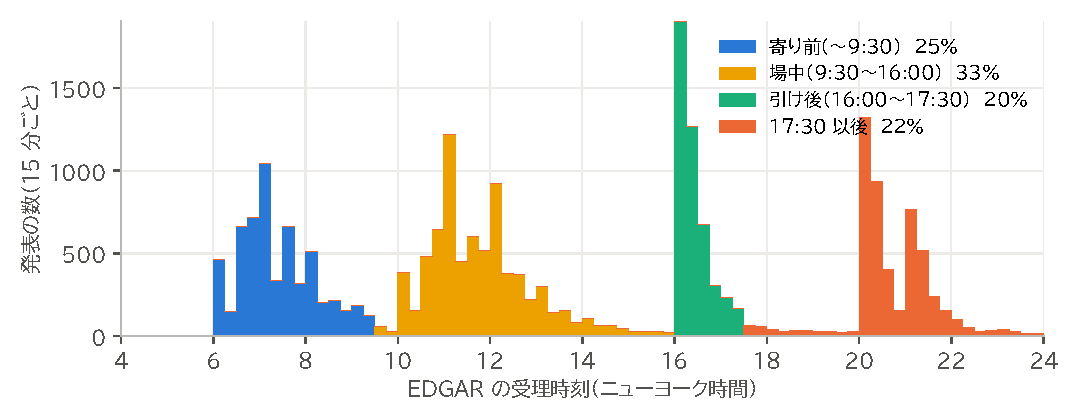
\includegraphics[width=0.9\linewidth]{timing.pdf}
\caption{受理時刻の分布（23,056 本）。4 つの山が約 4 時間ずれて対になっている。}
\label{fig:timing}
\end{figure}

受理時刻の分布（\figref{fig:timing}）には 4 つの山があり、寄り前（6〜8 時）と場中（10〜13 時）、引け後（16 時台）と 17:30 以後（20〜21 時）が、それぞれ約 4 時間ずれて対になっていた。多くの会社が、プレスリリースを配信してから数時間後に 8-K を提出するためである。主な窓（反応の日の前日の終値から翌日の終値まで）は、どちらの場合も配信の後の値動きを含む。

\chapter{データと点数}\label{ch:scorers}

\section{決算発表の取得}

SEC EDGAR から、\SP{} の構成銘柄（期間中に一度でも入った 668 社）の 8-K のうち Item 2.02 を含むものを取得した。SEC の求めに従い、User-Agent に連絡先を入れ（実行時の環境変数で渡し、保存しない）、毎秒 8 回以下に抑えた。H06 の 6,209 本と点数 5,429 本は新しい表に移し、件数と費用（3.31 ドル）が記録と一致することを確かめた。

\begin{table}[H]
\centering
\caption{決算発表のデータ。}
\small
\begin{tabular}{lr}
\toprule
取得した 8-K（2015 年 1 月〜2026 年 8 月） & 28,447 \\
本文が取れたもの & 28,108 \\
数値の驚き（SUE）が計算できたもの & 24,598 \\
取得にかかった時間（2015〜2023 年の 22,295 本） & 約 2.5 時間 \\
\bottomrule
\end{tabular}
\end{table}

\section{5 つの点数の付け方}

\begin{table}[H]
\centering
\caption{点数の付け方。時間はこの PC（GPU は RTX 5050 Laptop 8GB）での合計。}
\small
\begin{tabular}{p{2.4cm}p{7.2cm}p{3.6cm}}
\toprule
方法 & 中身 & 費用・時間 \\
\midrule
gpt-4o-mini & H06 と同じ質問。ガイダンスの変更・見通し・語調（$-2$〜$+2$）とリスクの種類 & 3.31 ドル（H06 で計算済み） \\
ChronoGPT & 発表の前の年末の版。選択肢の確率を、中身のない文章での確率で割って較正 & 0 円（8.3 時間） \\
辞書 & Loughran--McDonald。発表の年より後に加わった語は使わない & 0 円（6 分） \\
FinBERT & 先頭の 200 文の、肯定 $-$ 否定の確率の平均 & 0 円（4.2 時間） \\
TF-IDF＋リッジ & 四半期ごとに、それより前に窓が閉じた発表の反応で学び直す（事前登録の後） & 0 円（14 分） \\
\bottomrule
\end{tabular}
\end{table}

\section{ChronoGPT の環境}

ChronoGPT-Instruct の 2014〜2024 年末の 11 の版を取得した（\code{工房/LLM/chrono/}）。

\begin{itemize}
\item 元の重み（fp32、7.4GB）は 8GB の GPU に載らないので、bf16（3.7GB）に変換して保存した。元のファイルのハッシュは公開値と一致した。
\item 2022 年末の版でも、今の米国大統領を「Bill Clinton」と答える。指示の学習のデータが 2000 年より前の内容に限られているためで、知識を問う使い方には向かない。
\item 較正しないと、良い発表にも悪い発表にもガイダンスを 9 割以上「引き下げ」と答える癖がある。中身のない文章で測った癖で割る「文脈による較正」を標準にした。
\item 点数付けを速くする工夫を 2 つ入れた。選択肢の前の文章を 1 回だけ計算する、頭が同じ選択肢をまとめる。1 本 3.2 秒が 1.1 秒になり、結果は公式の計算と $10^{-7}$ 以下で一致した。
\item 版を切り替えるとき、前の版を GPU に残したまま次を読み込むと、メモリが溢れて 4 倍遅くなった。前の版を外してから読むように直した。
\end{itemize}

% ============================================================
\part{実験 2：事前登録したイベントの評価}
% ============================================================

\chapter{事前登録}\label{ch:prereg}

標本 A は、H06 で翌月のリターンについて一度見た期間である。結果を見てから手順を選ぶ余地をなくすため、株価の反応を一度も計算しないうちに、次のものを 1 つのコミット（\code{2df746e}）に固定して GitHub にプッシュし、その後に 1 回だけ実行した。

\begin{itemize}
\item 事前登録の文書（\code{preregistration.md}）：標本、変数、検定、判定の基準、副次の分析 S1〜S4、頑健性の確認 R1〜R7、実装の細部
\item 評価のコード（\code{run.py}）：作ったデータでだけテストしたもの
\item 使う点数の番号と、その設定のハッシュ
\end{itemize}

\begin{table}[H]
\centering
\caption{主な検定の設計。}
\small
\begin{tabular}{lp{10.4cm}}
\toprule
目的変数 & 反応の日の前日の終値から翌日の終値まで（2 取引日）の超過リターン（セクター ETF との差）。上下 1\% で丸める \\
主な説明変数 & gpt-4o-mini の合成点数（語調＋見通し＋ガイダンス、標準化） \\
統制 & SUE、売上の驚き、辞書・FinBERT・TF-IDF の点数、発表前 21 日の超過リターン、時価総額の対数、セクターと年・四半期の固定効果 \\
標準誤差 & 反応の日ごとにまとめる \\
置換の対照 & 同じ反応の日の中で点数を入れ替えて 1,000 回 \\
判定 & t 検定と置換の両方で片側 $p<0.05$ なら「支持」 \\
\bottomrule
\end{tabular}
\end{table}

丸めとコロナの時期の影響を見るため、丸めなし・幅を変えた丸め・順位の版・コロナの月を除いた版を、頑健性の確認（判定には使わない）として事前登録に入れた。

\chapter{結果}\label{ch:e2result}

\begin{verdict}
\textbf{支持。}標本 A（2023 年 11 月〜2026 年 8 月、5,374 本、527 の発表日）で、gpt-4o-mini の合成点数の係数は 1 標準偏差あたり $+120$bp（95\% 区間 $+95$〜$+145$bp、$t=9.41$）。置換の対照の片側 $p=0.001$（1,000 回で実際を超えたのは 0 回）。
\end{verdict}

\begin{figure}[H]
\centering
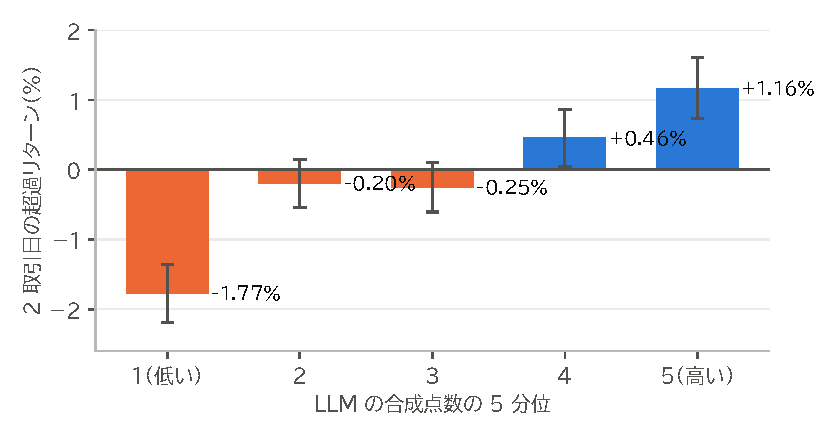
\includegraphics[width=0.6\linewidth]{quintile.pdf}
\caption{合成点数の 5 分位ごとの、2 取引日の超過リターン（探索の図）。}
\end{figure}

\begin{figure}[H]
\centering
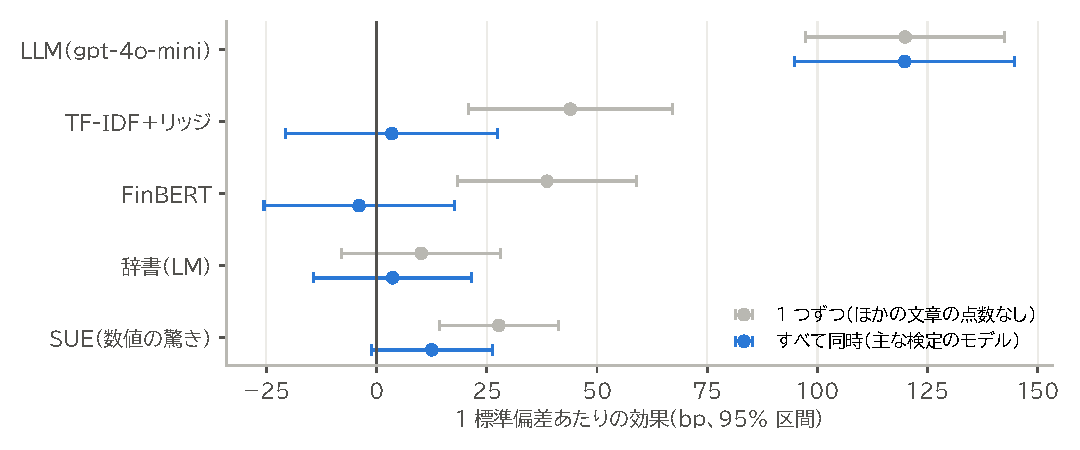
\includegraphics[width=0.9\linewidth]{compare.pdf}
\caption{点数ごとの効果。灰はほかの文章の点数を入れずに 1 つずつ、青はすべて同時（探索の図）。}
\label{fig:compare}
\end{figure}

\begin{figure}[H]
\centering
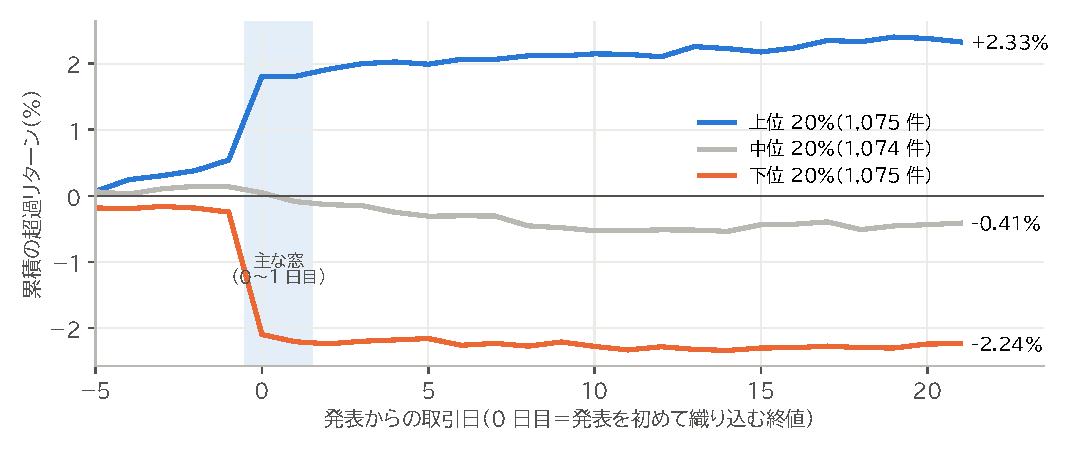
\includegraphics[width=0.9\linewidth]{car.pdf}
\caption{合成点数の上位・中位・下位 20\% の累積の超過リターン（探索の図）。}
\label{fig:car}
\end{figure}

\begin{figure}[H]
\centering
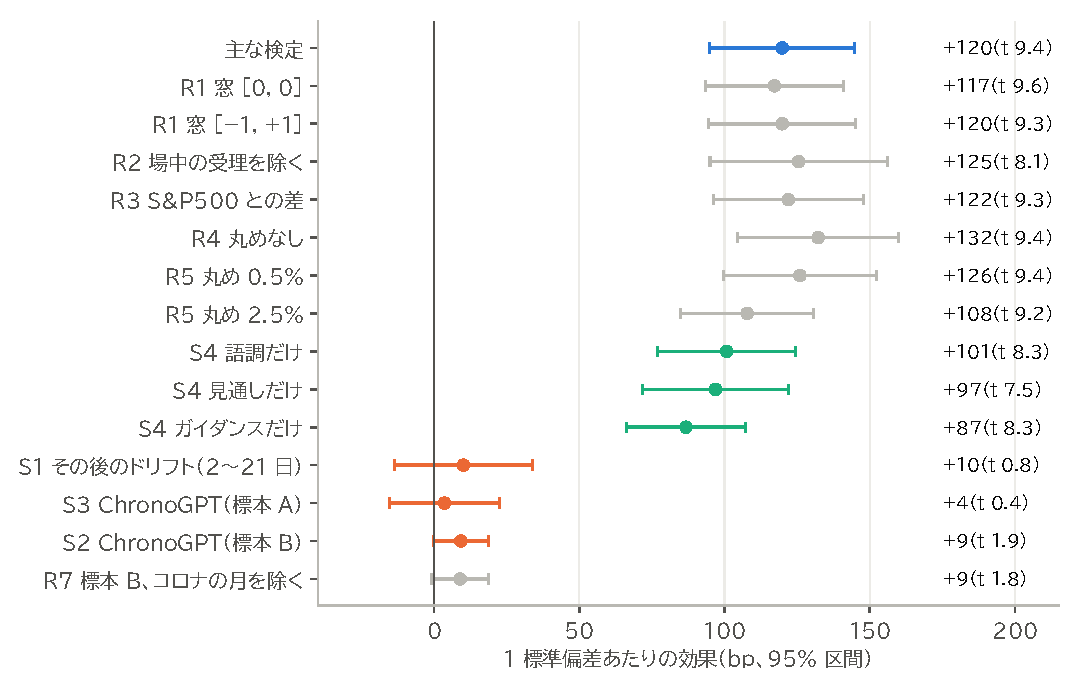
\includegraphics[width=0.9\linewidth]{forest.pdf}
\caption{主な検定（青）、頑健性（灰）、語調・見通し・ガイダンスの 1 つずつ（緑）、ドリフトと ChronoGPT（橙）。}
\label{fig:forest}
\end{figure}

\begin{itemize}
\item \textbf{点数の順に反応が並ぶ}：5 分位の平均は $-1.77\%$、$-0.20\%$、$-0.25\%$、$+0.46\%$、$+1.16\%$。
\item \textbf{LLM を使わない方法の情報をほぼ含む}（\figref{fig:compare}）：1 つずつなら TF-IDF（$+44$bp）、FinBERT（$+39$bp）、SUE（$+28$bp）も効くが、LLM と同時に入れると文章の 3 つの方法はほぼ 0 になる。LLM は 1 つずつでも同時でも $+120$bp。
\item \textbf{反応は 2 日で出尽くす}（\figref{fig:car}）：その後の 2〜21 日目のドリフトは有意でない（S1、$+10$bp、$t$ 0.8）。
\item \textbf{語調・見通し・ガイダンスは、どれも単独で強く効く}（S4、$+87$〜$+101$bp）。
\item \textbf{頑健}：窓、場中の受理、比べる指数、丸めの有無と幅、順位の版のどれでも、$t$ は 7.5〜9.6（\figref{fig:forest}）。
\item \textbf{ChronoGPT は弱い}：標本 A で $+4$bp（$t$ 0.4）、標本 B（2016〜2023 年、14,204 本）で $+9$bp（Holm の補正の後 $p=0.089$）。
\end{itemize}

\chapter{考察}\label{ch:e2disc}

\section{LLM は読めるが、儲けには使えない}

gpt-4o-mini は、決算発表文から「市場がどう受け取るか」を、辞書や FinBERT より正確に読み取れた。Siano（2025）の「LLM の測度は、辞書や LLM でない機械学習の 3 倍、発表の短い期間のリターンを説明する」と合う。一方、反応は 2 日のうちに出尽くし、点数が手に入るときには株価はすでに動いている（Wu ほか 2025 と合う）。H06 で翌月のリターンを説明できなかったことと矛盾しない。

\section{BLM にとっての意味}

BLM のビューは「これから先のリターンの見込み」なので、発表への反応を説明する点数をそのままビューにしても、価値は生まれない。総合報告書 1 からの問い「LLM のビューは BLM に追加の価値を生むか」への答えは、今の時点では「数値予想では生まない。文章の読み取りは正確だが、それが効くのは発表の瞬間だけで、月次のビューには生かせない」である。

\section{限界}

\begin{itemize}
\item 数値の驚きの統制が弱い（アナリストの予想がなく、前年同期との差で測った）。LLM が本文の「予想を上回った」を読んでいるなら、効果の一部は「文章から数値の驚きを読む力」である。
\item 主な標本は約 3 年（527 の発表日）。
\item 受理時刻は配信時刻ではない。場中の受理を除いても、窓を広げても結果は変わらなかった。
\item ChronoGPT の弱さは、モデルの弱さか、質問の形の弱さか区別できない。
\end{itemize}

% ============================================================
\part{関連の検討}
% ============================================================

\chapter{共分散のノイズ除去（X01）}\label{ch:x01}

BLM の共分散 $\Sigma$ は、約 460 銘柄を 252 日で推定している。銘柄の数が日数より多いので、標本共分散は逆行列がとれず、ノイズが大きい（\figref{fig:x01noise}）。今の BLM は Ledoit--Wolf の縮小推定を使っている。『ファイナンス機械学習』（López de Prado）の Marcenko--Pastur のノイズ除去と比べた（LLM は使わない、2016〜2026 年の 127 か月）。

\begin{figure}[H]
\centering
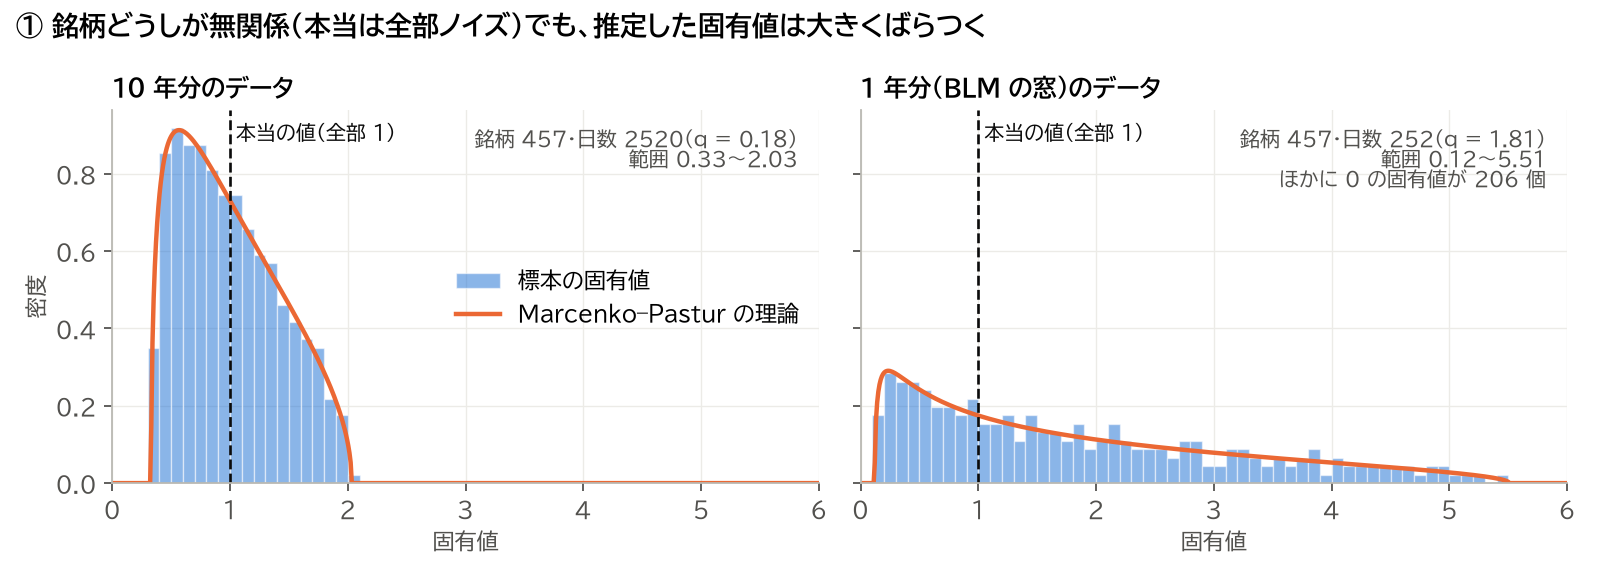
\includegraphics[width=0.95\linewidth]{x01_1_noise_only.png}
\caption{銘柄どうしが無関係な作ったデータでも、推定した固有値は大きくばらつく（1 年分では 0.12〜5.5 に広がり、206 個が 0）。}
\label{fig:x01noise}
\end{figure}

\begin{figure}[H]
\centering
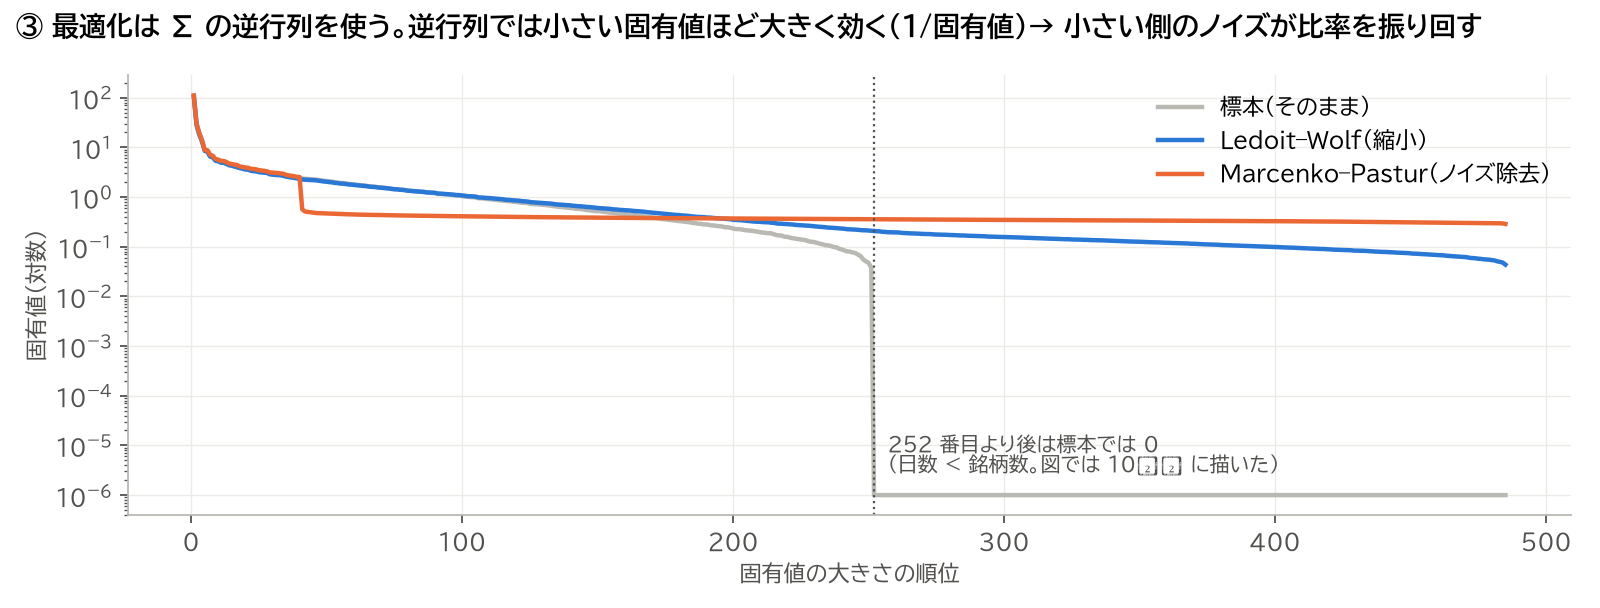
\includegraphics[width=0.95\linewidth]{x01_3_spectrum.png}
\caption{推定ごとの固有値。最適化は逆行列を使うので、小さい側のノイズが比率を振り回す。}
\end{figure}

\begin{table}[H]
\centering
\caption{翌月の実際のリスク（年率）。}
\small
\begin{tabular}{lrrr}
\toprule
& 標本 & Ledoit--Wolf（今の BLM） & Marcenko--Pastur \\
\midrule
制約のない最小分散 & 14.4\% & 11.3\% & \textbf{10.4\%} \\
空売りなしの最小分散 & 10.5\% & \textbf{10.5\%} & 10.6\% \\
BLM の最適化（TE の上限 3\%）：実際の TE & 4.8\% & \textbf{4.5\%} & 4.7\% \\
\bottomrule
\end{tabular}
\end{table}

\begin{itemize}
\item 制約のない最適化では、ノイズ除去がはっきり効く。
\item 空売りの禁止や TE の上限があると、制約そのものがノイズによる賭けを抑えるので、差はほぼ消える。\textbf{BLM の共分散は今の Ledoit--Wolf のままでよい。}
\item どの推定でも、実際の TE は上限 3\% の約 1.5 倍になった。H04 の実績の TE 4.2\% と合う。BLM の結果は、上限ではなく実際の TE で報告する。
\item 実際の株価では、Marcenko--Pastur が信号として残す固有値が平均 42 個と多い。銘柄ごとにノイズの大きさが違い、理論の前提が成り立たないためである。
\end{itemize}

\chapter{道具と計算環境}\label{ch:tools}

\section{外部のモデルと連携する道具}

同じ依頼を複数のモデルに出して比べる作業が増えたので、工房の道具を整えた。

\begin{itemize}
\item \code{LLM/ask.py}：OpenAI・Codex・Gemini・Gemini Deep Research・ローカルの LLM に質問する。ウェブ検索、PDF の添付、長い推論の裏での実行、モデルごとの答えと実行記録の保存に対応した。
\item \code{LLM/refcheck.py}：文献の実在、題名、著者を arXiv・OpenAlex・Crossref で照合する。今回の 4 者の調査の誤りは、すべてこれで見つかった。
\item スキル \code{llm-panel}：同じ依頼を 3 者に出して比べる手順をまとめた。
\end{itemize}

\section{計算の時間と外注の検討}

\begin{table}[H]
\centering
\caption{今回の計算（この PC）。}
\small
\begin{tabular}{lr}
\toprule
決算発表の取得（22,295 本） & 約 2.5 時間 \\
ChronoGPT の点数（28,108 本） & 8.3 時間 \\
FinBERT の点数（28,108 本） & 4.2 時間 \\
実験 2 の評価（TF-IDF の学習を含む） & 14 分 \\
API の費用（今回の追加分） & 0 ドル（gpt-4o-mini の点数は H06 のもの） \\
\bottomrule
\end{tabular}
\end{table}

ChronoGPT の点数付けのような GPU の作業は、RunPod や Vast.ai で GPU を時間単位で借りれば、数ドルで数倍〜10 倍速くできる見込みである。大学の RTX 3080 ×4 を SSH で使う案もある。どちらも、点数を付ける発表の一覧を書き出し、結果を DB に取り込む機能を足せば使える（\code{やること.md} の D1）。

% ============================================================
\part{まとめ}
% ============================================================

\chapter{課題と今後の計画}\label{ch:future}

この章は、本書を GPT（gpt-5.6）と Gemini（gemini-3.1-pro-preview）に読ませ、同じ依頼で独立に立案させた計画と、Claude の下書きを比べてまとめた（\code{資料集/03\_方針と文献調査/今後の計画/}）。2 者が挙げた文献は、すべて実在と著者を照合した。

\section{今の課題}

\begin{enumerate}
\item \textbf{実験 2 を、結果を見ていない発表で再現していない}（GPT）。主な標本は約 3 年（527 の発表日）で、しかも H06 で一度見た期間である。同じ標本を統制やプロンプトを変えて分析し直しても、新しい確認にはならない。
\item \textbf{数値の驚きの統制が弱い}（3 者）。アナリストの予想がないので、LLM が文章の中の「予想を上回った」「見通しを引き上げた」という数値の情報を読んでいるだけかもしれない。
\item \textbf{発表の時刻と標本の重複が監査されていない}（3 者）。受理は配信より遅れることがあり、8-K の訂正（8-K/A）や同じ日の複数の提出も確かめていない。
\item \textbf{先読みのない比べる相手が弱い}（3 者）。ChronoGPT の弱さが、モデルの限界か、ゼロショットの使い方の限界か区別できない。
\item \textbf{発表への反応と、投資の価値がつながっていない}（3 者）。ドリフトは有意でなく、BLM のビューにする根拠がない。
\item \textbf{試す設定が増えるほど、偶然の当たりを拾う}（GPT）。主な検定、頑健性、探索を分け、試した設定をすべて記録する必要がある。
\end{enumerate}

\section{次の段階の問い}

\begin{verdict}[主な問い]
gpt-4o-mini の点数が示した説明力（1 標準偏差あたり $+120$bp）は、結果を見ていない新しい発表でも再現するか。
\end{verdict}

副次の問いは、(1) ガイダンスの数値などで統制を強めても残るか、(2) 株価に触れない中立のプロンプトでも同じ点数になるか、(3) 先読みのない ChronoGPT の埋め込みは、ゼロショットや TF-IDF を超えるか、(4) 発表の後に、売買の費用を上回るドリフトが残るか、の 4 つである。

\section{前向きの再現は、12 月上旬に結果が出る}

前向きの検証は、2027 年 2 月まで待つ必要があるとして一度やめた（\chapref{ch:plan}）。しかし実験 2 で強い結果が出た今は、同じ標本の分析を重ねるより、新しい発表での再現のほうが価値が高い（GPT の指摘）。しかも、待つ期間は短くて済む。件数だけから見積もると（株価の反応は見ていない）、今の決算シーズン（2026 年 10 月 15 日〜11 月 30 日）だけで約 450 本・発表日 29 日がある。実験 2 の標準誤差から、120bp の効果なら片側 5\% で検出できる確率は約 86\%（80bp なら約 57\%）で、\textbf{結果は株価がそろう 12 月上旬に出る}。

\begin{table}[H]
\centering
\caption{前向きの標本の大きさと検出力の見込み（2025 年の同じ時期の件数と、実験 2 の標準誤差から計算）。}
\small
\begin{tabular}{lrrrrr}
\toprule
期間 & 発表 & 発表日 & 標準誤差 & 120bp & 80bp \\
\midrule
10 月 15 日〜11 月 30 日（1 シーズン） & 約 450 & 約 29 & 約 44bp & 86\% & 57\% \\
＋1 月 15 日〜2 月 28 日（2 シーズン） & 約 950 & 約 75 & 約 30bp & 99\% & 84\% \\
\bottomrule
\end{tabular}
\end{table}

\section{次の実験}

\begin{longtable}{p{2.6cm}p{11.6cm}}
\toprule
\textbf{実験} & \textbf{内容} \\
\midrule
\endfirsthead
\bottomrule
\endfoot
\textbf{1. 前向きの再現}（最優先、GPT） & \textbf{方法}：10 月下旬に、手順（実験 2 と同じ回帰・統制・判定）、対象（2026-10-15〜11-30 の受理）、開ける日を事前登録する。主な点数は H06 と同じプロンプト。\\
& \textbf{基準}：t 検定と置換の両方で片側 $p<0.05$ なら「再現した」。検出力が足りずに有意でないときは、「失敗」ではなく「判定不能」とする。\\
& \textbf{費用・時間}：API 1〜3 ドル。作業 2〜3 日と、シーズンの終わりまでの待ち。\\
& \textbf{次の判断}：再現すれば、統制の強化と仕組みの分解に進む。しなければ、実験 2 は期間に依存した結果として報告する。1〜2 月のシーズンを足すかは、今の時点で別に事前登録するかを決める（結果を見てから足すと、見ながら標本を増やすことになる）。\\
\midrule
\textbf{2. 監査と数値の統制}（3 者） & \textbf{方法}：重複（8-K/A、同じ日の複数の提出）を一覧にする。受理と配信のずれを、時間帯ごとに選んだ発表で手作業で照合する。発表文からガイダンスの数値（売上・EPS の見通し）を規則で抽出し、前回の見通しとの差を統制に加える。抽出は 100 本程度を人手で確かめる。\\
& \textbf{基準}（GPT の案）：反応の日の誤りが 5\% 以下、数値の抽出の精度が 90\% 以上。統制を強めても、前向きの標本で LLM の係数が残るか。既存の標本 A での分析は「探索」とする。\\
& \textbf{費用・時間}：2〜4 週間、API は使っても 5 ドル以内。\\
& \textbf{次の判断}：係数が大きく縮めば「文章から数値の驚きを読んだ効果」、残れば「数値以外も読んでいる」。\\
\midrule
\textbf{3. 中立のプロンプト}（GPT） & \textbf{方法}：株価や予測に触れない質問を事前に固定し、前向きの標本と標本 A に付ける。\\
& \textbf{基準}（GPT の案）：元の点数との順位相関が 0.8 以上で、前向きの標本でも係数が正で有意なら、測り方は安定とする。\\
& \textbf{費用・時間}：API 3〜6 ドル、1 週間。\\
\midrule
\textbf{4. ChronoGPT の埋め込み＋回帰}（3 者） & \textbf{方法}：最後の層（1,536 次元）を取り出し、各時点より前に窓が閉じた発表だけでリッジ回帰を学習する（He ほか 2025）。2016〜2023 年で、事前登録してから評価する。\\
& \textbf{基準}：同じ統制の下で、TF-IDF を入れても係数が正で、二つの検定で $p<0.05$。\\
& \textbf{費用・時間}：GPU で約 9 時間（大学の GPU か、時間単位の借用で 10 ドル以内）。実装 1〜2 週間。\\
& \textbf{次の判断}：成功すれば「先読みのない LLM の表現にも価値がある」。失敗しても gpt-4o-mini の結果は否定せず、小さなモデルの限界として分けて報告する。\\
\midrule
\textbf{5. ドリフトの関門}（GPT） & \textbf{方法}：実際の発表日の構造で、2〜21 日目のドリフトの検出できる最小の効果を計算する。前向きの標本と合わせて評価する。\\
& \textbf{基準}：ドリフトが二つの検定で有意で、95\% 区間の下限が売買の費用を上回るときだけ、順位の戦略・等リスク・BLM を同じ実際の TE と費用で比べる。それ以外では BLM を実行しない。\\
& \textbf{補足}：時価総額や文章の長さで分けてドリフトを探す案（Gemini）は、分けるほど偶然の当たりを拾うので、関門の外の「探索」として報告するだけにする。\\
\end{longtable}

\section{関門を通ったときの BLM への入れ方}

ドリフトの関門（実験 5）を通った場合、点数を BLM に入れる形は、これまでの実験でほぼ決まっている。どの部分も、LLM に数値を言わせない。

\begin{itemize}
\item \textbf{点数から期待リターンへ}：過去のイベントで、点数とその後のリターンの関係（較正の傾き）を測り、それで換算する（Grinold の $\alpha=\mathrm{IC}\cdot\sigma\cdot z$ の形）。
\item \textbf{不確かさ $\Omega$}：LLM の回答のばらつきではなく、過去の当たり具合で決め、$\Sigma$ に比例させる（H04 で設計どおりに動いた形）。当たらない信号は、採用率が自動で 0 に近くなる。
\item \textbf{相対ビューとベータの中立化}：同じセクターとの差のビューにし、能動ベータを 0 にする制約を置く（H03 で、相対ビューだけではベータの傾きが消えなかったため）。
\item \textbf{ビューを持つ期間}：ドリフトが続く期間だけビューを持ち、その後は外す。
\end{itemize}

\section{まだ株価に入っていない情報の候補（未検証）}\label{sec:candidates}

実験 2 で、LLM は決算発表文を正確に読めるが、その内容は 2 日で株価に入り切ることが分かった。BLM の価値につなぐには、LLM が「まだ株価に入っていない情報」を取り出せる必要がある。その候補を挙げる。\textbf{どれもまだ試していない。}どれを選ぶかは、前向きの再現とドリフトの関門の結果を見てから決め、選んだものは事前登録してから評価する。

\begin{longtable}{p{2.7cm}p{6.0cm}p{5.4cm}}
\toprule
\textbf{候補} & \textbf{考え方} & \textbf{データと注意} \\
\midrule
\endfirsthead
\bottomrule
\endfoot
\textbf{ゆっくり読まれる文書} & 10-K や 10-Q のリスクの記述や経営者による分析（MD\&A）は、決算発表文より長く、提出も遅く、注目されにくい。株価への織り込みが遅い可能性がある & EDGAR から無料で取れる。文書が長いので、gpt-4o-mini の費用は発表文より大きい。ChronoGPT は文脈が短く、全文は読めない \\
\midrule
\textbf{会社をまたぐ波及} & ある会社の決算の内容が、取引先や同業の株価に遅れて効く。投資家は、関係の深い他社の情報に注意を払いきれない & Yılkı（2026、arXiv:2606.29290、査読前の単著）は、10-K の MD\&A の FinBERT の埋め込みをサプライチェーンの関係で広げた信号が、\SP{} の 255 社（2011〜2025 年）で月次のリターンを予測すると報告している（要旨の範囲で確認、Newey--West の $t$ $-2.64$）。取引関係のデータは DB にない。10-K の主要な顧客の開示などから作る必要がある \\
\midrule
\textbf{セクター単位の集約} & 多くの会社の発表文から、業種全体の見通しやガイダンスの変化をまとめる。個々の会社の驚きはすぐ織り込まれても、業種全体の流れは遅れて効くかもしれない。BLM は、セクターや資産クラスの単位のビューと相性が良い & 既存の点数を集計するだけなので、追加の費用はない。セクターは 11 しかなく、月数も限られるので、検出力は低い（H05 と同じ問題） \\
\midrule
\textbf{リスクの側に使う} & 期待リターンではなく、不確かさが増える出来事（ガイダンスの取り下げ、リストラ、訴訟など）を読み、その銘柄の $\Sigma$ や $\Omega$ を大きくする。X01 で、実際の TE が上限の約 1.5 倍になった（リスクの変化に推定が追いつかない）問題にもつながる & H06 の gpt-4o-mini の点数には、すでにリスクの種類（\code{risk\_flags}）がある。評価は、リターンではなく、予測したリスクと実際のリスクの当たり具合（実現 $\div$ 予測、QLIKE）で行う \\
\end{longtable}

関門を通らなかった場合も、これらは次の実験の候補になる。そのときの結論は、「LLM は予言者としては価値がなく、読み手としては優秀だが、決算発表文の読み取りは BLM の価値にはならない」となる。これも、検証の確かさを目的とするこの研究にとっては、十分な結論である。

\section{スケジュール}

\begin{table}[H]
\centering
\caption{残りの期間の計画。}
\small
\begin{tabular}{p{2.4cm}p{6.6cm}p{4.6cm}}
\toprule
時期 & 作業 & 判断点 \\
\midrule
10 月下旬 & 前向きの再現の事前登録、重複の確認、株価の更新の仕組み、片づけ（取り下げ論文の引用、古い資料） & 手順を固定できたか \\
11 月 & 監査とガイダンスの数値の抽出、中立のプロンプト、ChronoGPT の埋め込みの実装、検出力の計算 & 抽出の精度が基準を満たすか \\
12 月上旬 & 10〜11 月の発表を取得・点数化し、株価を更新して、前向きの再現を 1 回だけ実行 & 再現したか（支持／支持されず／判定不能） \\
12 月中旬〜1 月 & ChronoGPT の埋め込みの検定、統制を強めた分析、ドリフトの関門 & 先読みのないモデルでも読めるか。BLM に進むか \\
2〜3 月 & 関門を通れば BLM の比較。通らなければ、候補（\secref{sec:candidates}）から 1 つを事前登録して試す。最終報告 & 結論を確定 \\
\bottomrule
\end{tabular}
\end{table}

費用は、API が 5〜10 ドル、GPU の借用は必要なときだけ 10 ドル以内の見込みで、これまでの約 10 ドルと合わせても予算（約 300 ドル）を大きく下回る。共分散の窓の比較（X02）は、主な分析を遅らせない範囲で行う。

\section{やらないこと}

\begin{itemize}
\item LLM に翌月のリターンを数値で予想させること（H02 で固有の IC が $-0.004$）。
\item 新しいモデル（gpt-5.x、gemini-3.x）での点数付け（評価期間の株価を知っている恐れがある）。
\item 同じ標本で多くのプロンプト・窓・統制を試し、最も良いものを主な結果にすること。
\item 今の点数を、そのまま月次の BLM のビューにすること。
\item 有料のアナリスト予想や分足の株価を前提にすること。
\end{itemize}

\section{リスクと未解決の問い}

\begin{itemize}
\item 知識の期限は、個々の文章や企業を覚えていないことの保証ではない。
\item 無料のデータだけでは市場の予想を再現できず、「数値以外を読んだ」という主張には限界が残る。
\item 前向きの標本は 1 シーズンでは小さく、効果が半分なら検出できない可能性が高い。
\item API のモデルの中身が変わると、点数が再現できなくなる恐れがある。モデルの版、答え、設定、ハッシュを保存して対処する。
\item \textbf{「LLM が従来の 3 倍正確に読めるのに、なぜドリフトがないのか」}（Gemini）。市場がすでに同じ水準の読み取りを瞬時に行っているのか、別の理由なのかは未解決である。
\end{itemize}


\chapter{結論}\label{ch:conclusion}

総合報告書 1 からの問い「LLM のビューは、Black-Litterman モデルや単純な統計に追加の価値を生むか」に、本書の作業は次のように答えた。

\begin{enumerate}
\item \textbf{LLM に数値のリターンを予想させても、価値はない。}予想は入力の写しで、固有の予測力は検出できず、BLM に入れても偶然と区別できない。プロンプトを工夫しても、フィードバックしても変わらなかった。
\item \textbf{LLM は、決算発表文を読む力では、従来の方法をはっきり上回る。}事前登録した検定で、発表への株価の反応を、辞書・FinBERT・TF-IDF・数値の驚きを超えて説明した（1 標準偏差あたり $+1.2\%$、$t$ 9.4）。
\item \textbf{しかし、その読む力は、取引や月次の BLM のビューには結びつかない。}反応は発表の 2 日で出尽くす。
\end{enumerate}

LLM の価値を BLM に生かすには、「発表の後もしばらく株価に織り込まれない情報」を LLM が取り出せることを示す必要がある。今の結果は、その情報が少なくとも gpt-4o-mini の発表文の点数には見られないことを示している。

次の一歩は、実験 2 の結果を、結果を見ていない 2026 年 10〜11 月の決算発表で再現することである（12 月上旬に結果が出る）。

% ============================================================
\part{付録}
% ============================================================

\appendix

\chapter{ブランチとコミット}\label{app:git}

\begin{table}[H]
\centering
\caption{本書の作業のブランチ（すべて GitHub にプッシュ済み。強制プッシュはしていない）。}
\small
\begin{tabular}{p{5.6cm}p{8.4cm}}
\toprule
ブランチ & 内容 \\
\midrule
\code{research/llm-blm-hypotheses} & 仮説の設計書 \\
\code{experiment/H01-verification}〜\code{H07-feedback-llm} & 仮説ごとの実験（前のブランチから順に分けた） \\
\code{research/llm-blm-results-report} & 実験結果レポートと、別のモデルによる確認 \\
\code{feature/earnings-events} & 設計、実装、データ、X01、事前登録（\code{2df746e}）、実験 2 の結果と報告書 \\
\bottomrule
\end{tabular}
\end{table}

\chapter{資料の一覧}\label{app:docs}

\begin{longtable}{p{6.4cm}p{7.6cm}}
\toprule
\textbf{資料} & \textbf{中身} \\
\midrule
\endfirsthead
\bottomrule
\endfoot
\code{資料集/02\_実験/実験1\_仮説の検証/}\newline LLM-BLM\_実験仮説 & 7 つの仮説の設計書（26 ページ） \\
\code{資料集/02\_実験/実験1\_仮説の検証/}\newline LLM-BLM\_実験結果レポート & H01〜H07 の結果（30 ページ） \\
\code{資料集/02\_実験/実験2\_決算発表文/} & 実験 2 の報告書（18 ページ）と図 \\
\code{設計.md} & 新しいアーキテクチャの設計 \\
\code{やること.md} & 次にやることの一覧 \\
\code{experiments/E2\_event\_reaction/} & 事前登録、評価のコード、結果 \\
\code{experiments/X01\_covariance\_}\newline\code{denoise/} & 共分散の比較と、ノイズ除去の解説 \\
\code{資料集/03\_方針と文献調査/設計方針/} & 3 者の方針と比較 \\
\code{資料集/03\_方針と文献調査/文献調査/} & 4 者の文献調査、照合の結果、比較 \\
\code{資料集/03\_方針と文献調査/まとめ/} & 文献調査と設計方針の PDF・PPTX（10 月 17 日朝の時点のもの。前向きの検証などは本書の方針で置き換えた） \\
\end{longtable}

\chapter*{参考文献}
\addcontentsline{toc}{chapter}{参考文献}

\begin{itemize}\small
\item Cao, S., Jiang, W., Xu, H. (2026). Seeing the Goal, Missing the Truth: Human Accountability for AI Bias. NBER WP 35142; arXiv:2602.09504.
\item Chen, S., Green, T. C., Gulen, H., Zhou, D. (2024). What Does ChatGPT Make of Historical Stock Returns? arXiv:2409.11540.
\item He, S., Lv, L., Manela, A., Wu, J. (2025). Chronologically Consistent Large Language Models. arXiv:2502.21206.
\item He, S., Lv, L., Manela, A., Wu, J. (2025). Instruction Tuning Chronologically Consistent Language Models. arXiv:2510.11677.
\item Huang, A. H., Wang, H., Yang, Y. (2023). FinBERT: A Large Language Model for Extracting Information from Financial Text. Contemporary Accounting Research 40(2).
\item Jagannathan, R., Ma, T. (2003). Risk Reduction in Large Portfolios: Why Imposing the Wrong Constraints Helps. Journal of Finance 58(4).
\item Kim, A. G., Muhn, M., Nikolaev, V. V. (2024). Financial Statement Analysis with Large Language Models. arXiv:2407.17866（2025 年 2 月に取り下げ）.
\item Kolari, J. W., Pynnönen, S. (2010). Event Study Testing with Cross-Sectional Correlation of Abnormal Returns. Review of Financial Studies 23(11).
\item Lee, Y., Kim, Y., Kim, S., Lee, Y. (2025). LLM-Enhanced Black-Litterman Portfolio Optimization. arXiv:2504.14345.
\item Lopez-Lira, A., Tang, Y., Zhu, M. (2025). The Memorization Problem: Can We Trust LLMs' Economic Forecasts? arXiv:2504.14765.
\item López de Prado, M. (2020). Machine Learning for Asset Managers. Cambridge University Press.
\item Loughran, T., McDonald, B. (2011). When Is a Liability Not a Liability? Journal of Finance 66(1).
\item Siano, F. (2025). The News in Earnings Announcement Disclosures: Capturing Word Context Using LLM Methods. Management Science 71(11).
\item Wu, Y., Akin, E. M., Martineau, C., Grégoire, V., Veneris, A. (2025). Extracting the Structure of Press Releases for Predicting Earnings Announcement Returns. arXiv:2509.24254.
\item Yılkı, A. (2026). Supply Chain Propagation of Textual Signals: LLM Embeddings and Cross-Sectional Return Predictability. arXiv:2606.29290（査読前）.
\end{itemize}

\end{document}
